\chapter{Introducción a la filosofía de la ciencia}
\label{cha:filosofiaciencia}

Estás en una carrera de Ciencias, rodeado de Científicos que hacen cosas
científicas, pero ¿qué es exactamente la ciencia?
¿Por qué la astronomía es una ciencia pero la astrología no?
¿A qué se dedican los científicos?
¿Es el método científico la única forma de hacer ciencia?
¿Un conocimiento científico es más confiable que un conocimiento no científico?
Todas estas preguntas son las que discuten los filósofos de la ciencia, y tratar
de responderlas y debatirlas nos brinda un mejor panorama de la naturaleza misma
de esta disciplina.

Para este capítulo ten en cuenta que las herramientas de la filosofía no son
las mismas que las de la ciencia.
La principal diferencia con los otros cursos de nuestra carrera es que aquí no
hay una respuesta definitiva a las preguntas que se plantean, y que el progreso
se logra mediante la discusión y la dialéctica: alguien propone una idea, otro
la critica, y así sucesivamente hasta llegar a un consenso, aunque este no sea
definitivo.

\section{Los orígenes de la ciencia}
\label{sec:losorigenesdelaciencia}

Para ponernos en contexto es importante conocer los orígenes de la ciencia, así
será más fácil entender por qué funciona como lo hace en la actualidad.

\subsection*{La ciencia en la antigüedad}
\label{sub:cienciaenlaantiguedad}
Desde la antigua Grecia, los filósofos se preguntaban por las causas del mundo.
Tal es el caso de \index{Aristóteles}{Aristóteles} (384--322 a. C.), quien
propuso muchas teorías físicas basándose en acertijos conceptuales y
razonamientos lógicos, pero sin experimentación ni
observación\cite{Shields2023}.
Su \index{física}{\emph{física}} se basaba en la idea de que la naturaleza busca
siempre la economía y la perfección; por ende sus teorías no fueron muy
acertadas.
Por ejemplo, él afirmaba que los cuerpos caen con una velocidad proporcional a
su peso.
A esta cosmovisión se le conoce como \emph{aristotelismo}, y fue la base del
conocimiento científico hasta el siglo \textsc{xvii}.

\begin{remember}
    \label{rem:aristotelismo}
    El \terminology[aristotelismo]{aristotelismo} es la cosmovisión que enfatiza
    la importancia de la lógica y la razón para entender el mundo.
\end{remember}

Parte central del aristotelismo fue la \index{teoría!geocéntrica}%
{teoría geocéntrica}, introducida por \index{Ptolomeo}{Ptolomeo} (90--168
d. C.). Esta teoría postula que la Tierra es el centro del universo y que todos
los demás cuerpos celestes giran alrededor de ella.

\begin{figure}[ht]
    \centering
    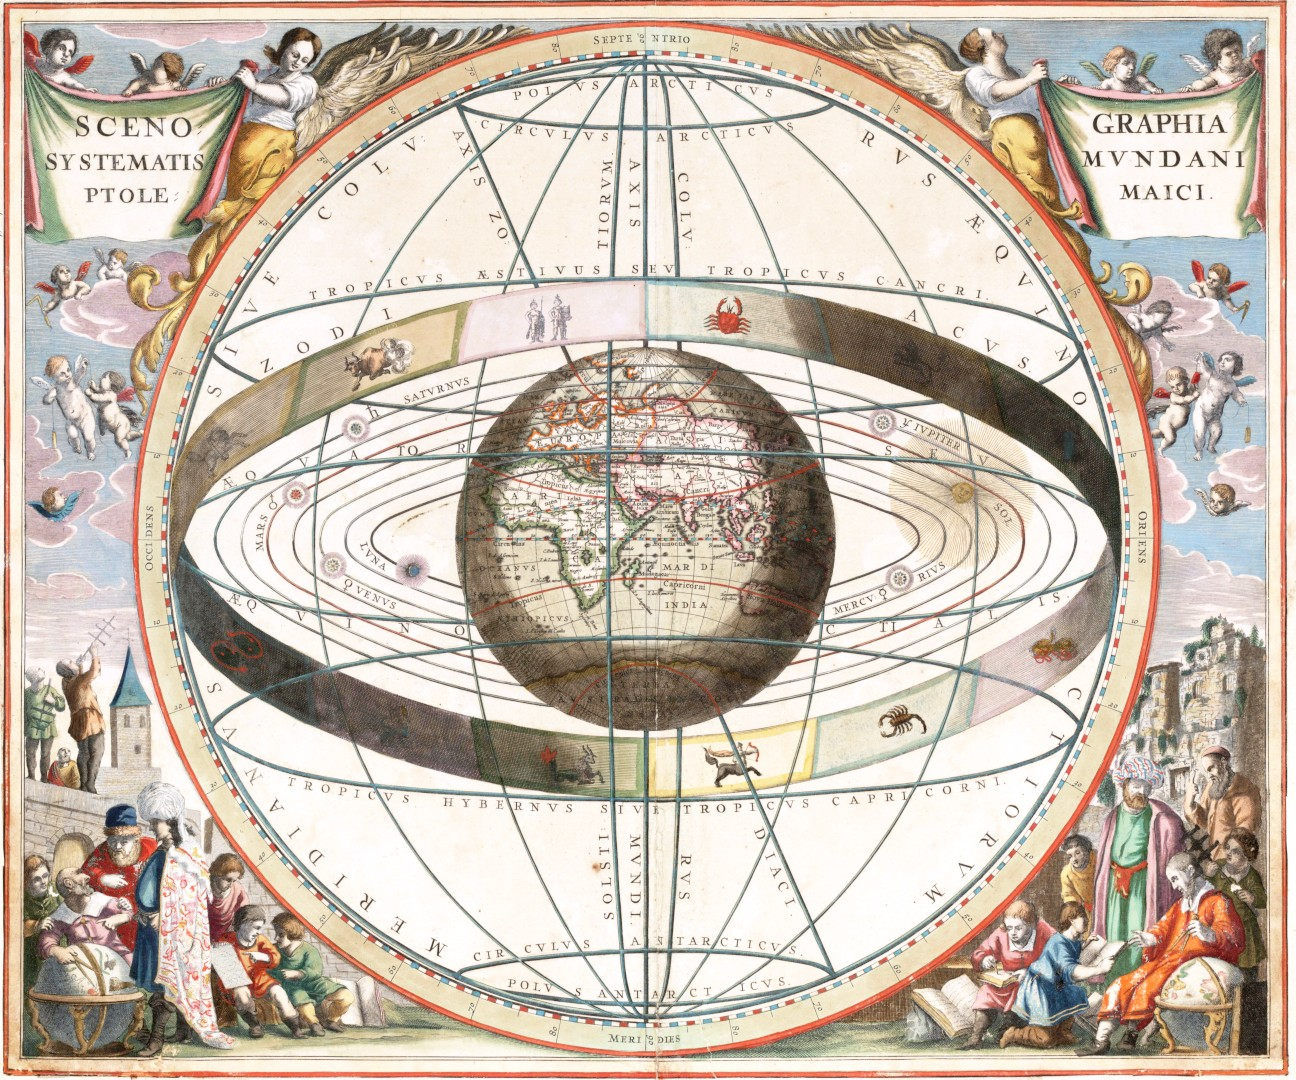
\includegraphics[width=0.8\linewidth]{img/Cellarius_ptolemaic_system}
    \caption{El sistema ptolemaico, en el que la Tierra es el centro del
        universo. Crédito: Loon, J. van (Johannes), aprox. 1611--1686 /
        Dominio público.}
    \label{fig:ptolemaico}
\end{figure}

\subsection*{La revolución científica}
\label{sub:larevolucioncientifica}
Fue hasta 1542 cuando el canónigo católico \index{Copérnico, Nicolás}%
{Nicolás Copérnico} (1473--1543) se atrevió a desafiar el aristotelismo
publicando su libro \emph{De revolutionibus orbium coelestium} (Sobre las
revoluciones de las esferas celestes), en el que propone que el Sol está fijo en
el centro del universo y que los planetas giran alrededor de él, dando lugar así
a la \index{teoría!heliocéntrica}{\emph{teoría heliocéntrica}}.

La teoría no fue bien recibida por la Iglesia, ni aún cuando su autor la dedicó
al Papa Pablo \textsc{iii}.
Más bien fue vetada de 1616 a 1835, pero en solo cien años se había convertido
en la teoría dominante gracias a los trabajos de \index{Galileo Galilei}{Galileo
    Galilei} (1564--1642) y \index{Johannes Kepler}{Johannes Kepler}
(1571--1630).
Kepler descubrió que los planetas se mueven en órbitas elípticas y no circulares
como creía Copérnico, y así resolvió el problema de la posición de Marte en el
cielo nocturno.
En cambio, Galileo apuntó su telescopio al cielo y descubrió que Júpiter tiene
cuatro lunas, que la Luna tiene montañas y cráteres, y que el Sol tiene manchas
entre otras cosas.

Galileo también hizo importantes contribuciones en otras áreas de la ciencia;
descubrió la \emph{ley de caída de los cuerpos}, que dice que todos los cuerpos
caen con la misma aceleración.
Según relata su discípulo Vivianni, esto lo demostró dejando caer dos bolas de
diferente peso desde lo alto de la Torre inclinada de Pisa
\cite{Viviani2019}.
Hasta entonces la lógica aristotélica era suficiente para explicar el mundo, la
experimentación era considerada una actividad de segunda clase, y las
matemáticas servían para describir objetos ideales pero no la realidad.
Galileo cambió todo esto, y por ello se le considera el primer científico
moderno.
Desafortunadamente, Galileo fue condenado por la Inquisición en 1633 por
defender a la teoría heliocéntrica, que para entonces era considerada herética
por contradecir la creación del mundo descrita en la Biblia.
Él pasó el resto de su vida bajo arresto domiciliario y se convirtió así también
en el ejemplo más famoso del conflicto entre ciencia y religión.

Luego de la muerte de Galileo, la ciencia entró en una etapa de rápido avance.
\index{Descartes, René}{René Descartes} (1596--1650), con su
\emph{mecanicismo}, propuso que el universo es como una
maquinaria de reloj en la que todo puede explicarse en términos del movimiento
y colisión de partículas.
Asimismo, en su \emph{Discurso del método} (1637) propuso que la ciencia debe
basarse en la razón y no en la autoridad, y que la experimentación y la
observación son las herramientas más importantes para el científico.

\begin{remember}
    \label{rem:mecanicismo}
    El \terminology[mecanicismo]{mecanicismo} es la cosmovisión según la cual
    el universo se comporta como una maquinaria determinista, y que puede ser
    explicada en términos del movimiento y colisión de partículas.
\end{remember}

Por su parte, \index{Newton, Isaac}{Isaac Newton} (1643--1727) propuso sus tres
leyes del movimiento y la ley de la gravitación universal, que explica la
atracción entre los cuerpos celestes.
Su obra maestra intitulada \emph{Philosophiae Naturalis Principia Mathematica}
(Principios matemáticos de la filosofía natural) se publicó en 1687, y fue el
marco teórico de referencia para la ciencia durante los siguientes 200 años.
Esta teoría sería extendida por muchos otros científicos para explicar más
fenómenos, como la mecánica de fluidos o la teoría electromagnética.

\begin{figure}[ht]
    \centering
    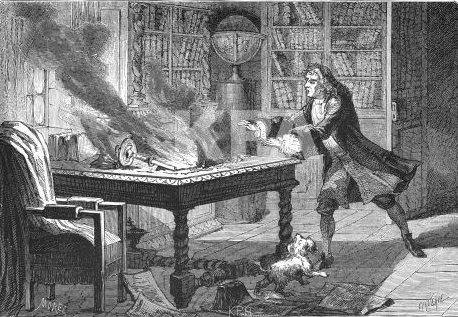
\includegraphics[width=0.8\linewidth]{img/Isaac_Newton_laboratory_fire}
    \caption{Isaac Newton en su laboratorio.
        Su mascota \emph{Diamond} tiró una vela sobre una mesa de papeles,
        quemando varios años de trabajo en el proceso.
        Crédito: Morel / Dominio público.
    }

\end{figure}

Durante un par de siglos se consideró que la teoría de Newton era esencialmente
correcta, y que los científicos sólo necesitaban rellenar meros detalles
técnicos para completar el cuadro.

\subsection*{La ciencia moderna}
\label{sub:lacienciamoderna}
En 1859, \index{Darwin, Charles}{Charles Darwin} (1809--1882) publicó su libro
\emph{El origen de las especies}, en el que propone la teoría de la evolución
mediante la selección natural.
Ya se sabía que las especies cambian con el tiempo si se seleccionan
artificialmente a los individuos más aptos para la reproducción en la
agricultura y la ganadería, donde se habían obtenido nuevas variedades de
plantas y animales más aptas para el consumo humano.
Darwin propuso que este mismo proceso ocurre en la naturaleza, donde las
especies co-evolucionan con su entorno y se adaptan a él.

A mediados del siglo \textsc{xix} el físico escocés \index{Maxwell, James}%
{James Maxwell} (1831--1879) descubrió que la luz es una onda electromagnética
que se propaga a la velocidad de la luz, unificando así las teorías de la
electricidad y el magnetismo.
Esto fue un gran avance, pero también un problema, pues las ecuaciones de
Maxwell entran en conflicto con la mecánica Newtoniana cuando se consideran
altas velocidades.
El final del siglo \textsc{xix} y el principio del \textsc{xx} fueron testigos
de invenciones increíbles como el teléfono, la radio, y el avión, pero también
de descubrimientos científicos que cimbraron la visión mecanicista del mundo.
En 1905, \index{Einstein, Albert}{Albert Einstein} (1879--1955) publicó su
\emph{teoría de la relatividad especial}, en la que propuso que el tiempo y el
espacio son relativos, y que la velocidad de la luz es la misma para todos los
observadores.

Por otro lado, apareció el problema de la \emph{radiación del cuerpo opaco}, que
desafiaba la física clásica al intentar comprender cómo un objeto caliente emite
radiación electromagnética.
Las predicciones clásicas indicaban que bajo ciertas condiciones este emitiría
radiación infinita, en clara contradicción con las observaciones experimentales.
Este problema fue resuelto por \index{Planck, Max}{Max Planck} (1858--1947) en
1900, quien propuso que la energía se emite en paquetes discretos llamados
\emph{cuantos}, dando origen a la \index{mecánica cuántica}{mecánica cuántica}.

En conjunto, la teoría de la relatividad y la mecánica cuántica revolucionaron
la física y la ciencia en general, disminuyendo la confianza en la teoría de
Newton y en el método científico clásico.
Ambas teorías son tan extrañas como exitosas, y han sido confirmadas por miles
de experimentos, pero aún así son difíciles de entender y de aceptar.

Para este entonces, la ciencia ya se hacía de forma colaborativa, las cartas
se publicaban en revistas científicas, y los científicos se reunían en
conferencias para discutir sus ideas.
Uno de estos grupos, el \index{círculo de Viena}{\emph{círculo de Viena}}, se
reunió a discutir la naturaleza de la ciencia, y en 1929 publicaron su
\emph{Manifiesto científico}, donde expresa la visión científica del mundo que
se basa en el empirismo, la lógica y el análisis del lenguaje.
El manifiesto propone que la filosofía se ocupe de clarificar los conceptos y
los criterios de la ciencia, y que rechace la metafísica como una pseudociencia
sin sentido.

\begin{remember}
    \label{rem:empirismo lógico}
    El \terminology[empirismo!lógico]{empirismo lógico} es una corriente
    filosófica que sostiene que el único conocimiento válido es el que se basa
    en la experiencia, la observación y la lógica.
    Una afirmación que no tiene contenido empírico o lógico es considerada
    \emph{metafísica}, y por lo tanto no tiene sentido.
\end{remember}

En 1936, \index{Turing, Alan}{Alan Turing} (1912--1954) publicó su artículo
\emph{On computable numbers, with an application to the Entscheidungsproblem},
en el que propuso un concepto matemático que eventualmente se convertiría en el
fundamento teórico de la computadora programable.
Su trabajo fue fundamental para el desarrollo de las computadoras y de la
computación moderna, sembrando la posibilidad de analizar a-priori el
comportamiento de un programa de computadora y sus limitaciones, aunque pasarían
varios años antes de que esto se hiciera realidad con la primera computadora
electrónica \emph{ENIAC} (Electronic Numerical Integrator and Computer) en 1946.

\begin{figure}[ht]
    \centering
    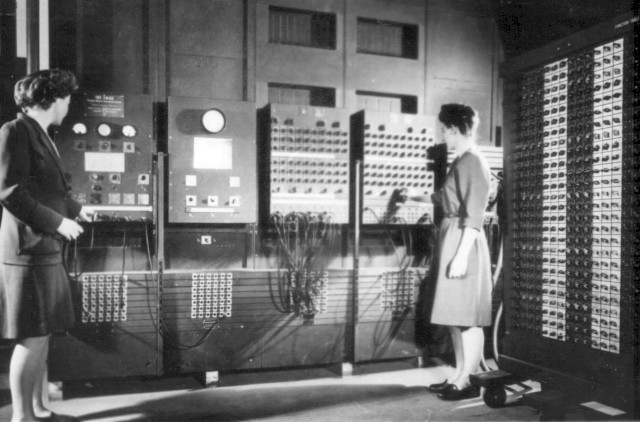
\includegraphics[width=0.8\linewidth]{img/Two_women_operating_ENIAC}
    \caption{Dos mujeres operando la computadora ENIAC.
        Crédito: U.S. Army Photo / Dominio público.
    }
\end{figure}

Para 1953, \index{Watson, James}{James Watson} (1928--) y
\index{Crick, Francis}{Francis Crick} (1916--2004) descubrieron la estructura
del ácido desoxirribonucleico (ADN), la molécula que contiene la información
genética de los seres vivos, dando inicio a la \index{biología!molecular}%
{biología molecular} que estudia los procesos biológicos en términos de las
moléculas que los componen.
Esta disciplina se ha desarrollado rápidamente gracias a la computación, que
permite simular y analizar los procesos biológicos a nivel molecular.
En 2003 se completó el \index{Proyecto Genoma Humano}{Proyecto Genoma Humano},
que consistió en secuenciar el ADN de un ser humano, y que ha permitido
entender mejor las enfermedades genéticas y desarrollar nuevos tratamientos
médicos.

\begin{figure}[ht]
    \centering
    \includegraphics[height=0.618\textheight]%
    {img/60_Jahre_DNA_01.jpg}
    \caption{Réplica del modelo de ADN de Watson y Crick.
        Crédito: Museum für Naturkunde Berlin.}
\end{figure}

\subsection*{La ciencia contemporánea}
El siglo \textsc{xx} fue testigo de la creación o formalización de disciplinas
como \index{economía}{economía}, \index{antrolopogía}{antropología},
\index{sociología}{sociología}, \index{psicología}{psicología}, y
\index{lingüística}{lingüística}.
En general, estas disciplinas se basan en el método científico, pero no son
ciencias naturales.
Por ejemplo, la sociología estudia la sociedad y la cultura, pero es mayormente
una ciencia observacional, pues no se pueden hacer experimentos con sociedades
humanas.

La tendencia actual es hacia la interdisciplinariedad, es decir, la
colaboración entre diferentes disciplinas para resolver un problema.
Una de estas ciencias artificiales que ha contribuido significativamente a
lograr esto es la \index{computación}{computación}, que estudia los fundamentos,
limitaciones y aplicaciones de la programación de computadoras.
La computación ha permitido simular y analizar fenómenos complejos que antes
eran inaccesibles.
Por ejemplo, la climatología estudia el clima de la Tierra, y para ello
simula el comportamiento de la atmósfera mediante modelos computacionales.
Estos métodos computacionales cuestionan la naturaleza misma de la ciencia.
¿Es válido un conocimiento científico que no se basa en la experimentación ni
en la observación, pero que es capaz de predecir el comportamiento de un
fenómeno observado?

\begin{remember}
    \label{rem:interdisciplinariedad}
    La \terminology{interdisciplinariedad} es la colaboración entre diferentes
    disciplinas para resolver un problema, y es la base de la ciencia moderna.
\end{remember}

Asimismo, la computación ha permitido el desarrollo de la inteligencia
artificial, que estudia la creación de máquinas inteligentes.
Esto ha llevado a la creación de programas de computadora que pueden jugar
ajedrez, conducir automóviles, diagnosticar enfermedades, pero más importante
para nuestra discusión, que hacer ciencia.
Estos programas de computadora se han usado exitosamente para descubrir
exoplanetas, predecir la estructura de proteínas, y descubrir nuevos materiales
entre otras cosas.
¿Se puede considerar \emph{conocimiento científico} a los resultados de estos
programas de computadora?

\section{Qué es la Ciencia}
\label{sec:queeslaciencia}

La ciencia intenta explicar, entender y predecir el mundo, pero también la
religión, la astrología, e incluso otras disciplinas como historia y filosofía.
La diferencia está en los métodos, a saber: la experimentación, observación y
construcción de teorías, pero definir exactamente qué es la ciencia es un
problema que ha ocupado a los filósofos durante siglos, y se conoce como el
\terminology[problema!demarcación]{problema de demarcación}.
A continuación veremos algunas propuestas que han surgido para resolver este
problema.

\subsection*{El empirismo}
\label{sub:elemprismo}
Durante la revolución científica, el filósofo inglés \index{Bacon, Francis}%
{Francis Bacon} (1561--1626) propuso, de forma retrospectiva, que la ciencia
debe basarse en la experimentación y la observación en su libro \emph{Novum
    Organum} (1620).
Para Bacon, la ciencia debe ser \emph{inductiva}, es decir, que debe partir de
muchas observaciones particulares para llegar a una conclusión general.
Esta es la idea central del \emph{empirismo}.
Así, cuando un empirista quiere entender algún fenómeno natural como la
combustión de la madera, debe observar muchos casos particulares de madera
quemándose para llegar a una conclusión general sobre el fenómeno.

\begin{remember}
    \label{rem:empirismo}
    El \terminology{empirismo} es la corriente filosófica que sostiene que el
    conocimiento se obtiene solo mediante la experiencia y la observación.
\end{remember}

Esto tiene mucho sentido para nosotros, pero en la antigüedad se creía que el
conocimiento se podía obtener mediante la razón y la lógica, y la
experimentación era relegada a un segundo plano.

Sin embargo este método tiene un problema: ¿cuántas observaciones son
suficientes para llegar a una conclusión general?
Si un turista visita a México, y más concretamente visita Tijuana, El Pinacate,
Cuatro Ciénegas, Real de Catorce, y el Paseo del Viejo Oeste de Durango, ¿puede
decir que todo México es un desierto?
¿Cuántos lugares debe visitar para poder decir que México es un país desértico?
¿Qué pasa si visita El Cañón del Sumidero, la Ciudad de México, o el Nevado de
Toluca?

\begin{figure}[ht]
    \centering
    
\includegraphics[width=0.8\linewidth]{img/Desierto_de_San_Luis_Rio_Colorado}
    \caption{El desierto de San Luis Río Colorado, Sonora, es una prueba
        contundente de que México es un país desértico.
        Crédito: Wikimedia Commons / CC BY-SA 4.0.}
\end{figure}

Quizás para este momento estés pensando que podemos corregir este problema si
además de observaciones también exigimos experimentos.
Desafortunadamente, esto no es suficiente, pues los experimentos no siempre dan
cuenta de las \emph{variables ocultas}.
Por ejemplo, si dejamos caer un martillo y una pluma desde la misma altura, el
martillo caerá más rápido, y estarías tentado a decir que los objetos pesados
caen más rápido que los ligeros.
Sin embargo, si hacemos el experimento en el vacío veremos que ambos caen con
la misma velocidad.
Esto es porque nuestro experimento no tomó en cuenta la resistencia del aire,
que es una variable oculta.
Este experimento al vacío ya fue llevado a cabo durante la misión
\emph{Apollo 15} en 1971, cuando el astronauta \index{David Scott}{David Scott}
\href{https://youtu.be/Oo8TaPVsn9Y}{ dejó caer una pluma y un martillo} en la
superficie lunar como homenaje a Galileo.

Si los experimentos no son suficientes, al menos podrías argumentar que por lo
menos sí son necesarios para hacer ciencia.
Esto tampoco es así, pues hay disciplinas que claramente son científicas pero
que no se basan en la experimentación, como es la astronomía.
Entonces, si la experimentación no es necesaria ni suficiente para describir a
un conocimiento como científico, ¿qué es lo que sí lo hace científico?

\subsection*{El falsacionismo}
\label{sub:elfalsacionismo}
El filósofo \index{Popper, Karl}{Karl Popper} (1902--1994) vivió en una de las
épocas más importantes de la ciencia moderna y, observando el éxito de Einstein
y Planck, se dio cuenta de que no todo conocimiento científico se crea de la
misma forma.
Él propuso una solución al problema de distinguir la ciencia de la no-ciencia
mediante el \terminology[falsacionismo]{falsacionismo}:
según Popper, una teoría \emph{científica} es aquella que, al menos en
principio, puede ser refutada mediante la experimentación.
Por ejemplo, la ley de caída de los cuerpos de Galileo es una teoría científica
porque si el día de hoy quisieras refutarla, bastaría con soltar dos bolas de
diferente peso desde una altura y ver que caen con distinta aceleración (siempre
que tomes en cuenta la resistencia del aire y otros factores).
Probablemente nunca lograrás refutarla, pero la mera posibilidad de hacerlo es
lo que cuenta; esta es la característica fundamental de una teoría científica.

La idea central del falsacionismo es muy simple y tiene mucho sentido,
después de todo, ¿qué sentido tiene una teoría que no se puede generalizar?
Encuentra una anomalía o contraejemplo y toda la teoría se cae.
Aquí además es importante considerar que en nuestra búsqueda de anomalías
\emph{la ausencia de evidencia no es evidencia de ausencia}.
Es decir, si no encuentras una anomalía no significa que no exista, sino que
no la has encontrado.
Así, mientras hayas intentado encontrarla y fracasado en el intento, tu teoría
es científica según Popper.

¿Y cómo es que esto nos permite distinguir entre ciencia y no-ciencia?
Consideremos las \terminology[pseudociencia]{pseudociencias}, que son
disciplinas que se hacen pasar por ciencia pero que no lo son.
La astrología tiene cierto parecido con la astronomía porque ambas estudian los
cuerpos celestes, pero la astrología es universalmente considerada una creencia
supersticiosa.
¿Puede el falsacionismo ayudarnos a distinguir entre la astronomía y la
astrología?
Veamos: los astrónomos hacen predicciones suficientemente vagas como para que
siempre sean ciertas, y cuando no lo son, simplemente inventan una explicación
ad-hoc para justificarlas, como por ejemplo, que su predicción no se cumplió
porque la persona no se leyó el horóscopo en el momento adecuado.
Entonces la astrología no es científica porque no puede ser refutada, y por lo
tanto es una pseudociencia.
¿Qué hay de la astronomía?
Los astrónomos hacen predicciones muy específicas, como por ejemplo, que el
próximo eclipse solar será visible en toda América del Norte el 8 de abril de
2024.
Si este eclipse no ocurre, entonces la teoría de la astronomía se cae, y por lo
tanto es una teoría científica.
Así ha ocurrido con muchas predicciones astronómicas, como la predicción de
\index{Edmond Halley}{Edmond Halley} (1656--1742) de que el cometa que lleva su
nombre volvería a ser visible desde la Tierra en 1758, lo cual ocurrió en la
fecha predicha.

\begin{figure}[ht]
    \centering
    
\includegraphics[width=0.8\linewidth]{img/creenciasdegente}
    \caption{Incluso algunas de las personas que se dedican a vender productos
        mágicos admiten que esas son creencias de gente ignorante.
        Tal es el caso de %
        \href{https://eldeforma.com/2020/04/08/mujer-explota-quedate-en-casa-quien-me-mantiene-huevos-para-curar/}%
        {una yerbera en Guanajuato} quien se viralizó tras
        realizar una entrevista para la televisión de forma por demás
        sincera.}
\end{figure}

\begin{remember}
    \label{rem:falsacionismo}
    El \terminology{falsacionismo} distingue ciencia y pseudociencia mediante
    la refutación de teorías científicas.
    Una teoría que nunca puede ser refutada ni siquiera en principio no es
    científica.
\end{remember}

Entonces, ¿es el falsacionismo la solución al problema de demarcación?
No tan rápido; hay dos problemas con esta propuesta.
En primera, suena muy extraño decir que los científicos \emph{inventan}
teorías y que se dedican a refutarlas; ciertamente eso no ocurre en la práctica.
Generalmente los científicos se dedican a \emph{construir} teorías de forma
paulatina mejorando la teoría anterior, y sólo cuando se encuentran varias
anomalías es que se dedican a refutarlas.
En efecto, el segundo problema es que en la práctica no es fácil ni conveniente
rechazar una teoría científica solo porque se encontró una anomalía.

Un ejemplo muy delicioso ocurrió en 1963, cuando un estudiante de Tanzania
llamado \index{Mpemba, Erasto}{Erasto Mpemba} (1950--) descubrió durante una
clase de hacer helados que el agua caliente se congela más rápido que el agua
fría.
Más tarde, en 1969, publicó un artículo en el que describía su
descubrimiento\cite{Mpemba1979}, pero los científicos no le creyeron porque
contradecía la teoría de la termodinámica.
La comunidad científica, lejos de abandonar la teoría de la termodinámica, se
dedicaron a buscar una explicación que encajara en la teoría, y en 2017 dos
equipos independientes de científicos publicaron artículos en los que explicaban
el fenómeno.

Independientemente de si Popper tenía razón o no, su propuesta de que la ciencia
tiene una característica fundamental que la distingue de la no-ciencia es muy
atractiva, pero bien podría ser falsa; después de todo, la ciencia está echa por
humanos de diferentes culturas y épocas, y las distintas disciplinas científicas
tienen diferentes métodos y objetivos.

\section{Los métodos científicos}
\label{sec:losmetodoscientificos}

A veces pareciera que los científicos inventan teorías de la nada, como que el
universo se expande o que los humanos evolucionaron de un ancestro común con los
chimpancés.
En realidad los científicos siguen un proceso muy largo y estrucuturado para
llegar a estas conclusiones en el que los conocimientos previos se van
acumulando y mejorando paulatinamente.
Los detalles varían de disciplina a disciplina, pero en general se basan en tres
métodos de razomiento: \emph{deducción}, \emph{inducción}, y
\emph{abducción}.

\subsection*{Deducción}
\label{sub:deduccion}
La deducción es un método de razonamiento que consiste en partir de premisas
generales para llegar a una conclusión.
Por ejemplo, si sabemos que todos los seres humanos son mortales, y que Mahoma
es un ser humano, entonces podemos deducir que Mahoma es mortal.
En lógica de primer orden, este razonamiento se puede expresar como sigue:
\begin{align*}
               & \mathit{HUMANO}(x) \Rightarrow \mathit{MORTAL}(x) & \text{(1)}        \\
               & \mathit{HUMANO}(\mathit{MAHOMA})                  & \text{(2)}        \\
    \hline
    \therefore & \mathit{MORTAL}(\mathit{MAHOMA})                  & \text{(de 1 y 2)}
\end{align*}

Este tipo de razonamiento es muy común en las matemáticas y la lógica;
probablemente antes de este curso ya lo habías usado en los cursos de
matemáticas.
Los razonamientos deductivos generalmente comienzan enunciando aquello que se da
por cierto (los \emph{axiomas}), y a partir de estos se derivan conclusiones
(\emph{teoremas}).

Los científicos utilizan la deducción para derivar predicciones de sus teorías,
a veces de forma tan natural que ni siquiera se dan cuenta.
Por ejemplo, la teoría de la evolución por selección natural dice que todos los
organismos se reproducen con variación y se adaptan a su entorno; los humanos
son organismos; por lo tanto, los humanos se reproducen con variación y se
adaptan a su entorno.

\begin{remember}
    \label{rem:deduccion}
    La \terminology{deducción} es un método de razonamiento que parte de
    premisas generales para llegar a una conclusión.
    Si las premisas son verdaderas, entonces la conclusión también lo es.
\end{remember}

La deducción no nos dice nada acerca de la validez de las premisas; así,
podríamos deducir que Juan toma tequila dadas las premisas de que todos los
mexicanos toman tequila y que Juan es mexicano.
Este razonamiento es válido, pero no es cierto porque las premisas son falsas.
A veces se suele comparar la lógica deductiva con el ajedrez: ahí no importa si
las piezas son de madera, plástico o las corcholatas que te sobraron de la
fiesta de anoche, lo que importa son las reglas del juego y lo que puedes
hacer con ellas.
De la misma forma, la lógica deductiva es un juego de palabras al que no le
importa el significado de estas; si las premisas son verdaderas y se siguen las
reglas de la lógica, entonces la conclusión también es verdadera.

La deducción se usa comúnmente en el ámbito científico para derivar
\emph{explicaciones} a partir de teorías.
Según el filósofo de la ciencia \index{Hempel, Carl}{Carl Hempel} (1905--1997),
todas las explicaciones científicas tienen la siguiente estructura:
\begin{description}
    \item[Explanandum] Existe un fenómeno que queremos explicar; generalmente
        es una observación particular.
    \item[Explanans] Para dar explicación al fenómeno, usamos nuestros
        conocimientos previos, que incluyen leyes generales y las condiciones
        iniciales específicas en las que ocurrió el fenómeno.
\end{description}

La explicación científica es, entonces, el razonamiento deductivo que trata al
fenómeno que queremos explicar como un teorema que se sigue de las leyes
generales y las condiciones iniciales.
Por ejemplo, si quiero explicar por qué la taza de café que dejé en la mesa se
enfrió, puedo apelar a la segunda ley de la termodinámica que dice que el calor
fluye de los cuerpos calientes a los fríos.
Dado que la taza de café estaba caliente rodeada de aire frío, puedo deducir que
el calor de la taza de café fluyó al aire, concluyendo así que la taza de café
se enfrió.
Normalmente no hacemos este razonamiento de forma consciente ni de manera tan
estructurada; en cambio, lo hacemos de forma natural y omitiendo muchos detalles
que consideramos obvios.
Así, para explicar por qué Juan está ebrio, simplemente decimos \emph{Juan tomó
    tequila}, y omitimos el resto de la deducción.

\begin{figure}
    \centering
    \begin{minted}{prolog}
% El tequila contiene alcohol.
contiene(tequila, alcohol).

% Una persona bebe una sustancia si esta está contenida
% en la bebida que la persona bebe.
beber(Persona, Sustancia) :-
    contiene(Bebida, Sustancia),
    beber(Persona, Bebida).

% Juan bebe tequila.
beber(juan, tequila).

% Una persona está ebria si bebe alcohol.
ebrio(Persona) :-
    beber(Persona, alcohol).

% ¿Está Juan ebrio?
consulta :- (
        ebrio(juan) -> writeln('Juan está ebrio')
        ; writeln('Juan no está ebrio')
    ),
    halt.
:- initialization(consulta).
\end{minted}
    \caption{Programa en Prolog que usa lógica deductiva para determinar si
        Juan está ebrio.
        Nuestra mente rara vez hace un razonamiento tan formal como lo requiere
        una computadora.}
\end{figure}

Sin embargo, nótese que este modelo de Hempel no distingue entre explicaciones y
predicciones: el mismo razonamiento deductivo que nos lleva a explicar por qué
la taza de café se enfrió también nos lleva a predecir que las tazas de café que
dejemos en al aire frío se enfriarán, o que Juan se embriagará cada vez que
tome tequila.

\subsection*{Inducción}
\label{sub:induccion}
La inducción es un método de razonamiento que consiste en partir de casos
particulares para llegar a conclusiones generales.
Al conjunto de casos particulares se le conoce como \emph{evidencia}, y a la
conclusión general se le conoce como \emph{hipótesis}.
Por ejemplo, en 1959 el médico pediatra Jérôme Lejeune (1926--1994) analizó los
cromosomas de nueve niños con síndrome de Down y encontró que todos ellos tenían
tres copias del cromosoma 21 en lugar de dos; esto lo llevó a concluir que el
síndrome de Down es causado por una copia extra del cromosoma 21%
\cite{Lejeune1959}.
Detengámonos un momento a reflexionar en esto: se analizaron 9 casos
particulares de 9 infantes particulares, pero llegó a una conclusión general que
se aplica a todos los seres humanos incluyendo a los que aún no han nacido.
¿Cómo es esto posible?

\begin{remember}
    \label{rem:induccion}
    La \terminology{inducción} es un método de razonamiento que parte de casos
    particulares para llegar a conclusiones generales.
\end{remember}

Ciertamente no siempre es posible generalizar a partir de observaciones
particulares.
A veces los científicos se equivocan al generalizar, como cuando el astrónomo
\index{Percival Lowell}{Percival Lowell} (1855--1916) observó canales en la
superficie de Marte y concluyó que eran obra de una civilización extraterrestre
avanzada.
Esto es porque en su experiencia todos los canales que había visto eran obra de
una civilización.
¿Qué tanto podemos generalizar a partir de observaciones particulares?
Cuenta la anécdota que un grupo de investigadores de la UAEM viajaba por los
campos del centro de México cuando vieron un rebaño de ovejas.
-- Todas las ovejas de este campo son blancas -- dijo el computólogo.
-- Corrección -- dijo el físico -- algunas ovejas de este campo son blancas.
-- No, no, no -- dijo el matemático -- existen algunas ovejas en este campo que
son blancas en al menos menos de uno de los lados.

\begin{figure}[ht]
    \centering
    
\includegraphics[width=0.8\linewidth]{img/oveja}
    \caption{No siempre podemos generalizar a partir de observaciones
        particulares y posiblemente incompletas.}
\end{figure}

En realidad, la inducción es más común de lo que parece; la usamos todo el
tiempo para hacer predicciones y es algo tan natural como necesario para poder
sobrevivir.
\begin{itemize}
    \item Desde que tienes memoria, la luna llena aparece cada 29 días, así que
          predices que la luna llena aparecerá cada 29 días en el futuro.
    \item Te quemaste con la llama de una vela de niño y ahora crees que todas
          las llamas queman.
    \item Sacaste tres manzanas podridas de la bolsa, así que supones que todas
          las demás manzanas están podridas y procedes a tirarlas a la basura.
    \item Un día decidiste viajar en la ruta 13 hacia la UAEM; ahora la usas
          todos los días porque supones que siempre llegará a la UAEM.
\end{itemize}

La inducción es, pues, encontrar patrones en los datos y generalizarlos.
Si a eso añadimos matemáticas o computación obtenemos la estadística y el
aprendizaje automático respectivamente; disciplinas muy poderosas en la ciencia
moderna.

Sin embargo, el razonamiento inductivo se basa en una suposición muy importante:
que situaciones nuevas serán similares a las que ya hemos experimentado, y que
la naturaleza sigue un patrón constante y predecible.
A esta hipótesis se le conoce como el \emph{Principio de Uniformidad}.
Sin este principio la inducción no tendría sentido, pues no podríamos
generalizar a partir de observaciones particulares: el principio de uniformidad
y la inducción son dos caras de la misma moneda.

\begin{remember}
    \label{rem:principio de uniformidad}
    El \terminology{Principio de Uniformidad} es la hipótesis de que la
    naturaleza sigue un patrón constante y predecible.
    Es equivalente al principio de inducción.
\end{remember}

La mayoría de las personas asumen que el principio de uniformidad es cierto
sin siquiera pensarlo, pero ¿cómo estamos seguros?
Si el Sr. Contreras (el \emph{escéptico}) te pide que demuestres la veracidad
del principio de uniformidad, ¿qué le responderías?
Tenemos de dos sopas para demostrar la veracidad del principio de uniformidad:
\begin{description}
    \item[Por deducción] Usemos el método de reducción al absurdo; aquí
        suponemos que el principio de uniformidad es falso y llegamos a una
        contradicción; como la lógica no admite contradicciones entonces el
        principio de uniformidad debe ser verdadero%
        \footnote{%
            los estudiantes que conozcan el
            \href{http://intrologic.stanford.edu/extras/resolution.html}%
            {\emph{principio de resolución}} entenderán que la reducción al
            absurdo es el método más general para demostrar la veracidad de
            cualquier proposición en lógica deductiva.
        }.
        Así, supongamos que el principio de uniformidad es falso.
        En un universo sin uniformidad el agua caliente a veces se congela y a
        veces se evapora, el fuego a veces quema y a veces enfría, la gravedad
        a veces atrae y a veces repele, y la ruta 13 a veces te lleva a la UAEM
        y a veces al reclusorio.
        Ciertamente es un mundo muy extraño y caótico, pero no produce ninguna
        contradicción lógica.
    \item[Por inducción] El principio de uniformidad nos ha permitido inventar
        cosas como el teléfono, el avión, los viajes espaciales y muchas cosas
        más, por lo tanto el principio funciona y es verdadero.
        Sin embargo, para el Sr. Contreras el hecho de que este principio haya
        funcionado \emph{en el pasado} no garantiza que funcionará \emph{en el
            futuro} a menos que asumamos el principio de la uniformidad… ¡pero
        eso es justo lo que queremos probar!
\end{description}
Como ambas formas de razonamiento son infructuosas entonces no podemos demostrar
la veracidad del principio de uniformidad.
A esta limitación se le conoce como el \emph{problema de la inducción de Hume},
propuesto por el filósofo escocés \index{Hume, David}{David Hume} (1711--1776),
y es uno de los problemas más importantes y activos de la filosofía de la
ciencia.

Algunos filósofos modernos como Peter Strawson argumentan que el principio de
uniformidad no sólo no se puede probar, sino que es un despropósito siquiera
intentarlo\cite{Strawson2012}.
Consideremos el siguiente argumento:
Si la Suprema Corte de Justicia de la Nación quiere establecer la
constitucionalidad de una ley, como por ejemplo prohibir a los hombres usar
pantalones, utiliza la constitución como base para determinar si la ley tiene
validez.
Pero si la Suprema Corte quiere establecer la constitucionalidad de la
constitución, ¿qué base utiliza?
Después de todo, si la constitución es la ley suprema, ¿tiene sentido usar a la
constitución para probar que la constitución es constitucional?
En este mismo sentido, el principio de inducción es una forma de razonar, y no
tiene sentido usar el razonamiento para probar la validez del razonamiento
mismo.

\subsection*{Abducción}
\label{sub:abduccion}
Hay ocasiones en las que más de una teoría puede explicar un fenómeno, y no
podemos decidir cuál es la verdadera.
La  \emph{abducción} consiste en descartar una a una las teorías que
consideramos que no son verdaderas hasta que sólo quede una.
Por ejemplo, si un día te despiertas con dolor de cabeza, fiebre, y dolor de
garganta, podrías pensar que te adulteraron la bebida en la fiesta de noche, que
tienes cáncer de garganta, que te propinaron una paliza mientras dormías, o que
simple y sencillamente te resfriaste.
¿Cuál de estas explicaciones debemos considerar como la correcta?
Probablemente lo que harías es descartar una a una las explicaciones que no
tienen sentido o sean muy improbables hasta que sólo quede una; eso es la
abducción.

Muchas veces este proceso no tiene una razón puramente lógica, sino que se basa
en ideas estéticas como la simplicidad, la elegancia, o la belleza.
Quizá la encarnación más famosa de la abducción es la \emph{navaja de Ockham},
propuesta por el filósofo inglés \index{Ockham, Guillermo de}{Guillermo de
    Ockham} (1285--1347), que dice que \emph{en igualdad de condiciones, la
    explicación más sencilla suele ser la correcta}.


\begin{remember}
    \label{rem:abduccion}
    La \terminology{abducción} es un método de razonamiento que consiste en
    descartar teorías según algún criterio hasta que sólo quede una.
    La \terminology{navaja de Ockham} es un principio estético que dice que
    \emph{en igualdad de condiciones, la explicación más sencilla suele ser la
        correcta}.
\end{remember}

¿Exactamente qué significa que una explicación sea más sencilla que otra?
Consideremos la construcción de la pirámide de Cuculcán en Chichén Itzá; hay
muchas teorías que intentan explicar cómo los mayas pudieron construir una
pirámide tan perfecta, que tiene una orientación tan precisa, y que además
tiene un significado astronómico.
Una de estas teorías dice que los mayas tenían ayuda de extraterrestres, y otra
dice que los mayas tenían conocimientos astronómicos muy avanzados.
¿Cuál de estas teorías es la más sencilla?
La oración “Los mayas construyeron la pirámide con ayuda de extraterrestres
usando tecnología avanzada” es muy sucinta y explica el fenómeno en cuestión,
pero introduce el problema de explicar cómo los extraterrestres llegaron a la
Tierra, cómo los mayas se comunicaron con ellos, y cómo los mayas obtuvieron
su tecnología avanzada; es decir, esta explicación \emph{sencilla} en realidad
es muy compleja, pues introduce más problemas de los que resuelve.

\begin{figure}[ht]
    \centering
    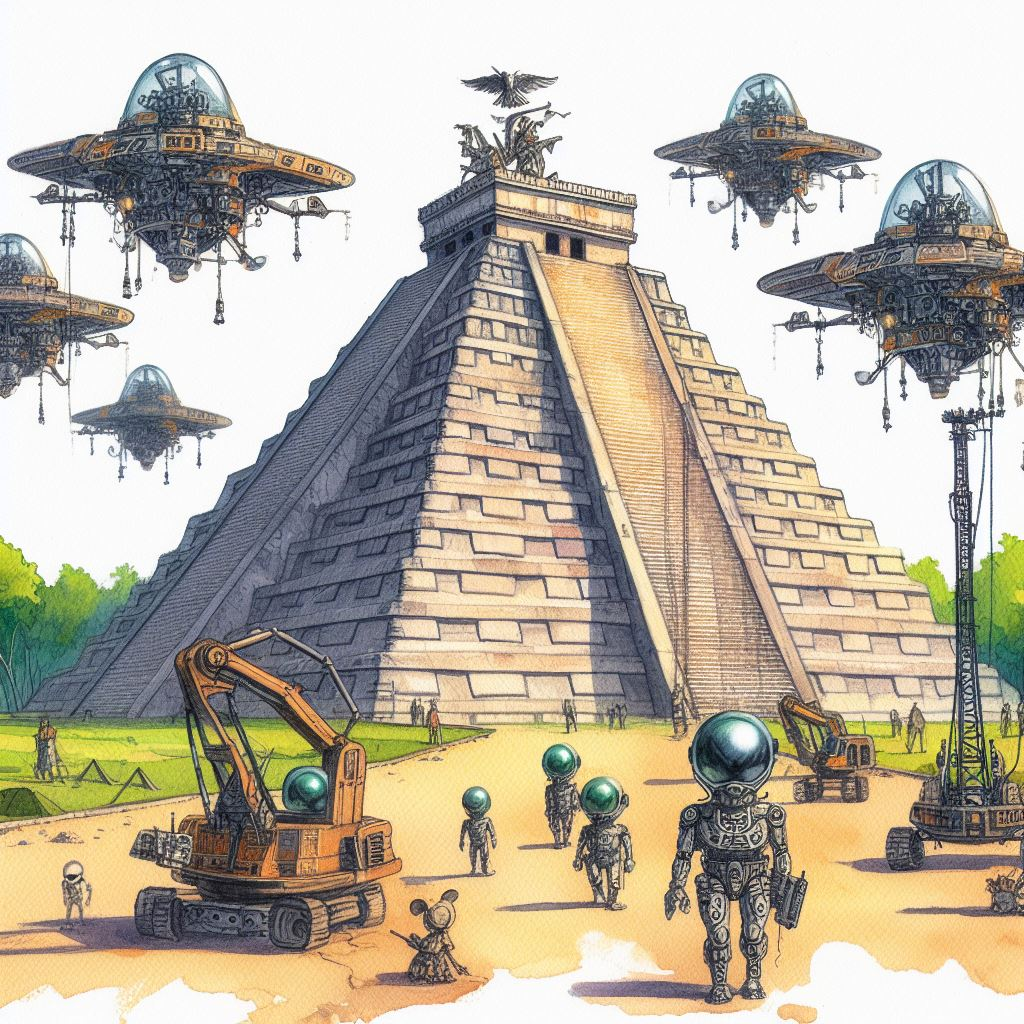
\includegraphics[width=0.8\linewidth]{img/chichenitza}
    \caption{Una explicación \emph{sencilla} para el misterio de la construcción
        de la pirámide de Cuculcán en Chichén Itzá.}
\end{figure}

Según el ejemplo anterior, a veces las explicaciones que parecen más complejas
en realidad son más sencillas por el simple hecho de que no introducen más
problemas de los que resuelven.
De hecho, a veces estas explicaciones “sencillas” suelen ser simples argumentos
\emph{ad ignorantiam}, es decir, que intentan rellenar un hueco en nuestro
conocimiento con una explicación que no tiene evidencia.

Ciertamente el universo no tiene ninguna razón lógica para ser sencillo ni
estético, pero existe evidencia para creer que hay cierta \emph{parsimonia} en
la naturaleza:
El agua fluye por el camino de menor resistencia, los átomos se organizan en
cristales geométricos de estructura regular, y las leyes de la física son
simples y elegantes.
El libro \emph{The Parsimonious Universe}\cite{Hildebrandt2012} relata a detalle
los esfuerzos de los científicos y matemáticos desde el Renacimiento para
identificar y describir las leyes básicas que subyacen a la forma de las formas
naturales, culminando con el cálculo de variaciones y la optimización matemática
como herramientas para entender la naturaleza.

Cabe mencionar que algunas personas consideran a la abducción como un caso
particular de la deducción en donde las ideas de simplicidad y elegancia se
expresan explícitamente como axiomas.
Es por eso que es común que cuando se habla de los métodos científicos se
mencione solo a la deducción (la razón) y la inducción (la evidencia), pero no
a la abducción (la estética).

\subsection*{El método científico}
\label{sub:elmetodocientifico}
A lo largo de la historia, varios filósofos y científicos (con mentes
filosóficas) han intentado describir un método general para hacer ciencia.
Me gustaría dedicar los siguientes párrafos a desmentir el gran mito del
\emph{método científico}, que según varios libros e incluso referencias
académicas como \cite{Crawford1990}, tiene algunos pasos bien definidos que
debes seguir y repetir para hacer ciencia, a saber:
\begin{description}
    \item[Observación.] Realiza una observación que te lleve a formular
        una pregunta;
    \item[Hipótesis.] formula una explicación (hipótesis) que pueda explicar la
        observación y responder a la pregunta;
    \item[Experimentación.] prueba la hipótesis realizando un
        experimento que se pueda repetir; analiza los datos del experimento y
        compara con la hipótesis y; finalmente,
    \item[Conclusión.] concluye si la hipótesis es correcta o no.
\end{description}
Cualquiera que tenga un poco de formación en filosofía de la ciencia (como tú,
oh querido lector) o bien que trabaje en un instituto de investigación, sabe que
este método es una simplificación exagerada difícil de aplicar en la práctica.
Como material de divulgación para niños está bien, pero no es real; y si eres de
la UAEM te invito a que le preguntes a tus profesores del Centro de
Investigación en Ciencias (CInC) cómo es que ellos hacen ciencia y los pasos que
siguen de este método.

El método científico es un mito que se ha popularizado gracias a los libros de
texto, pero un poco de reflexión nos hace ver que este método es tan común que
no es exclusivo de la ciencia: lo usan los bebés para aprender que los objetos
permanecen en su lugar aún cuando no los ven, lo usan los gatos para aprender
que cuando tiran un vaso de agua de la mesa este se rompe, y lo usan los
estudiantes de la UAEM para aprender que si no estudian reprobarán el examen.

En realidad, no existe método científico único ni general; tratar de definirlo
no solo es impositivo, sino que es equivalente a tratar de definir qué es la
ciencia misma, es decir, nos topamos con el \emph{problema de demarcación} del
que hablamos en la sección~\ref{sec:queeslaciencia}.
El filósofo argentino \index{Mario Bunge}{Mario Bunge} (1919--2020) abordó este
problema creando un catálogo de atributos que son comunes a varias disciplinas
científicas en \emph{La ciencia, su método y su filosofía}\cite{Bunge1996}, pero
no se exige que todas las disciplinas cumplan con todos los atributos.
Es como cuando haces un test de personalidad y te dicen que si sacas más de 50
puntos entonces tu personalidad es la de un tamal, pero si sacas menos de 50
puntos tu personalidad es la de una enchilada: no importa cuántos puntos saques,
tu personalidad es la misma.
De la misma manera una disciplina podría ser considera \emph{científica} si
cumple con cierta \emph{puntuación mínima} arbitraria dada por el catálogo de
Bunge.

\section{Las revoluciones científicas}
\label{sec:lasrevolucionescientificas}
A finales de los años 50, cuando el profesor universitario de Historia de la
Ciencia \index{Thomas Kuhn}{Thomas Kuhn} (1922--1996) recorría los pasillos de
la Universidad de Harvard, observó que los estudiantes de posgrado no hacen
ciencia como la hacían los científicos de la historia y que, lejos de seguir un
método científico impulsados por la curiosidad y la observación, estos se
dedicaban a resolver problemas técnicos de una forma más bien rutinaria.
Con base en estas y otras observaciones, Kuhn criticó la visión idealizada de la
ciencia que se tenía en su época en una influyente monografía de 1962
intitulada \emph{La estructura de las revoluciones científicas}\cite{Kuhn2005}.
Su estilo provocativo y polémico ha sido objeto de innumerables críticas y
defensas por parte de filósofos y científicos, y su obra se considera una de
las más influyentes de la filosofía de la ciencia del siglo XX.

\subsection*{La ciencia según el Círculo de Viena}
\label{sub:circulodeviena}
En la época de Kuhn, la ciencia se consideraba como un proceso en el que los
científicos iban descubriendo poco a poco nuevos conocimientos que se iban
añadiendo a los libros de texto.
Las conocimientos más nuevos son objetivamente mejores, pues corrigen y mejoran
a los conocimientos anteriores; así, la ciencia es un proceso lineal y
acumulativo que progresa hacia la verdad.
Esta forma de pensar era influenciada principalmente por el \emph{círculo de
    Viena} que mencionamos previamente en la sección~\ref{sub:lacienciamoderna}.

Para los miebros del círculo de Viena, la ciencia era una disciplina que está
por encima de las demás debido a su objetividad y racionalidad.
En lugar de responder a las preguntas científicas con opiniones subjetivas de
los expertos (como sí ocurre en filosofía y otras áreas) se usan métodos
objetivos como la observación y la experimentación.
En particular, cuando dos teorías científicas rivalizan, los científicos pueden
resolver el conflicto comparando las teorías con datos neutrales y objetivos.
El cómo se obtienen estos datos de manera neutral no es claro, pero el círculo
de Viena postula que estos datos existen y que los bandos en conflicto pueden
llegar a un acuerdo por medio de ellos y del pensamiento racional.

Otro tema importante para el círculo de Viena era el delimitar lo que se
considera relevante para la labor científica.
Por ejemplo, a diferencia de los filósofos, los científicos no se deben de
preocupar por entender la historia de la ciencia ni el contexto social en el que
se desarrolla, después de todo estos temas son irrelevantes si sólo importa la
objetividad y la racionalidad.
En efecto, el círculo de Viena distingue entre dos contextos en la ciencia:
\begin{description}
    \item[Contexto de descubrimiento.] Es el proceso por el cual los científicos
        obtienen sus ideas y formulan hipótesis.
        Este proceso es subjetivo carece de importancia.
    \item[Contexto de justificación.] Es el proceso por el cual los científicos
        justifican las ideas e hipótesis.
        Este proceso es puramente objetivo, y define a la ciencia misma.
\end{description}


\begin{remember}
    \label{rem:circulodeviena}
    Según el \terminology{círculo de Viena}, la ciencia se distingue de otras
    disciplinas por ser objetiva y racional.
    Según esta cosmovisión, el contexto histórico y social es irrelevante, y
    solo importa el contexto de justificación de las teorías científicas.
\end{remember}

Según esta distinción, a todos nos da igual que al químico \index{Friedrich
    August Kekulé}{Friedrich August Kekulé} (1829--1896) se le haya ocurrido la
estructura del benceno en un sueño donde una serpiente se mordía la cola (cosa
que realmente sucedió) o que la estructura se le haya aparecido un pan tostado,
lo importante es que pudo justificar su idea mediante experimentos rigurosos.
Así, cuando hablemos del benceno en un curso de química no mencionaremos el
sueño de Kekulé, sino que nos enfocaremos en los experimentos que justifican
su estructura.
Esta postura sigue algo vigente en la actualidad: los libros de texto rara vez
mencionan el folclor que rodea a los descubrimientos científicos, en parte por
razones pedagógicas, y en parte porque este folcore se considera irrelevante.

\begin{figure}[ht]
    \centering
    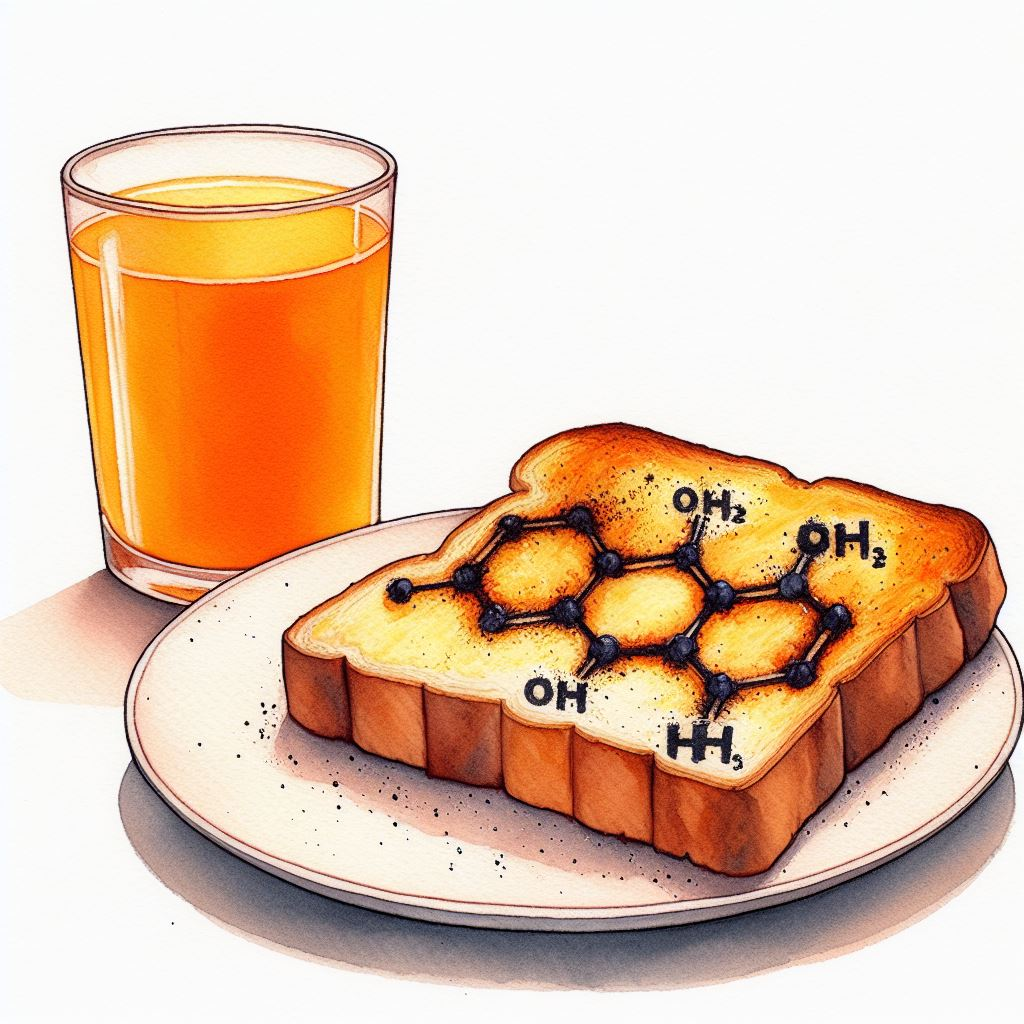
\includegraphics[width=0.8\linewidth]{img/formaciondehipotesis}
    \caption{Según el círculo de Viena no importa cómo se te ocurrió esa
        hipótesis, sino cómo la justificas.}
\end{figure}

\subsection*{La ciencia según Kuhn}

Desde su perspectiva de historiador de la ciencia, Kuhn notó que la cosmovisión
del círculo de Viena no concordaba con los hechos históricos.
Él estaba interesado en las \terminology[revolución científica]%
{revoluciones científicas} que ocurren cuando una teoría científica establecida
es reemplazada por una nueva, como cuando Darwin reemplazó la teoría de la
creación divina con la teoría de la evolución por selección natural, o cuando
Einstein reemplazó la teoría newtoniana de la gravedad con la teoría de la
relatividad general.
Las revoluciones científicas no son frecuentes, pero cuando estas ocurren
cambian el \terminology{paradigma} de la disciplina, es decir el conjunto de
creencias y valores compartidos por los científicos de un área.
Más formalmente, un paradigma consta de dos partes:
\begin{description}
    \item[Teorías.] Son las suposiciones fundamentales que los científicos de
        una disciplina comparten.
    \item[Ejemplares.] Son ejemplos concretos de problemas que han sido
        resueltos con éxito por medio de las teorías establecidas.
\end{description}
Así, el paradigma determina el modelo teórico de una disciplina, los problemas
se deben abarcar, cómo se deben plantear, con qué métodos se deben resolver y,
en general, el panorama completo de la disciplina.


Entre los periodos de revolución, los científicos trabajan en resolver problemas
técnicos del modelo establecido, explicando las anomalías que aparecen en los
datos sin cuestionar el paradigma mismo, como si se tratara de un rompecabezas.
A este periodo Kuhn lo denomina \terminology{ciencia normal}.
Es sólo cuando las anomalías se vuelven demasiado grandes que el modelo
establecido se cuestiona y entra en una crisis que culmina con la propuesta y
aceptación de un nuevo paradigma.

\begin{figure}[ht]
    \centering

    \begin{tikzpicture}[
            node distance=1cm,
            ellipsenode/.style={ellipse, draw, fill=Lavender},
            rectanglenode/.style={
                    rectangle,
                    draw,
                    minimum width=6cm,
                    minimum height=1.5cm,
                    fill=Gold
                },
            >=stealth,
            line width=1pt
        ]

        \node[rectanglenode] (pre) {Fase pre-científica};
        \node[ellipsenode, below=of pre] (acept) {Aceptación de un paradigma};
        \node[rectanglenode, below=of acept] (normal) {Fase de ciencia normal};
        \node[ellipsenode, below=of normal] (anom) {Aparición de anomalías};
        \node[ellipsenode, below=of anom] (nuevo) {Nuevo paradigma};
        \node[rectanglenode, below=of nuevo] (rev) %
        {Fase de revolución científica};

        \draw[->] (pre) -- (acept);
        \draw[->] (acept) -- (normal);
        \draw[->] (normal) -- (anom);
        \draw[->] (anom) -- (nuevo);
        \draw[->] (nuevo) -- (rev);
        \draw[->, dashed] (rev.east) to[out=0,in=0] (acept.east);
    \end{tikzpicture}

    \caption{Según Kuhn, la ciencia no es un proceso lineal y acumulativo, sino
        que se da en ciclos donde un paradigma establecido es reemplazado por
        uno nuevo, que no necesariamente mejora al anterior.}
\end{figure}

\begin{remember}
    \label{rem:paradigma}
    Un \terminology{paradigma} es el conjunto de creencias y valores compartidos
    por los científicos de un área.
    Este define la manera de hacer \terminology{ciencia normal} en dicha área.
    Solo cuando las anomalías se vuelven demasiado grandes el paradigma entra
    en crisis y ocurre una \terminology{revolución científica}.
\end{remember}

Esta manera de aceptar y rechazar paradigmas no totalemente racional ni objetiva
como postula el círculo de Viena, sino que es un proceso social y psicológico.
Esta idea es muy polémica y ha sido objeto de muchas críticas, pero tiene
bastante mérito cuando consideramos que la ciencia es una actividad humana y que
históricamente ha sido la presión social y política la que ha determinado el
paradigma dominante de una disciplina.

\subsection*{Los paradigmas, su inconmensurabilidad e irracionalidad}
Pero la cosa se pone peor, ya que el nuevo paradigma no es necesariamente mejor
que los anteriores, sino que a veces retoma ideas antiguas que habían sido
descartadas previamente.
Por ejemplo, Kuhn afirma que la teoría de la relatividad general de Einstein
tiene más parecido a la teoría aristotélica de la gravedad que a la teoría
newtoniana.
Entonces cabe cuestionarse si realmente la ciencia progresa hacia la verdad, o
si al menos existe una noción objetiva de verdad.

¿Realmente pueden dos teorías científicas rivales ser comparadas con datos
neutrales y objetivos?
Kuhn afirma que no, ya que lo que se considera verdadero depende del paradigma
mismo.
Por ejemplo, el concepto de \emph{masa} en la teoría de Newton tiene un
significado completamente distinto al concepto de \emph{masa} en la teoría de la
relatividad de Einstein, y al no haber un lenguaje común para comparar ambas
teorías concluimos que es imposible decidir cuál teoría es la verdadera.
A esto Kuhn le denomina la
\terminology[paradigma!inconmensurabilidad]{inconmensurabilidad} de los
paradigmas, y significa que el acto de aceptar un paradigma es más bien un acto
de fe que un acto racional.

\begin{figure}[ht]
    \centering
    
\includegraphics[width=0.8\linewidth]{img/actodefe}
    \caption{Según Kuhn, aceptar un paradigma científico es más bien un acto de
        fe guiado por la presión social y la psicología.}
\end{figure}

\begin{remember}
    \label{rem:inconmensurabilidad}
    La \terminology{inconmensurabilidad} de los paradigmas significa que no
    existe un lenguaje común para comparar teorías rivales, y por lo tanto no
    se puede decidir cuál teoría es la verdadera.
\end{remember}

En las ediciones posteriores de su libro, Kuhn suavizó un poco su postura y
aceptó que a veces los paradigmas pueden ser más o menos comparables, después de
todo si no fuesen en absoluto comparables entonces no habría necesidad de
revoluciones científicas.
Lo que sí están de acuerdo Kuhn y sus críticos es que la ciencia no tiene un
algoritmo para la elección de teorías.
Recordemos que un algoitmo es un conjunto instrucciones precisas que se siguen
paso a paso para realizar una tarea.
¿Qué forma más racional de elegir teorías hay que no sea un algoritmo diseñado
con base en la lógica y la evidencia?
Aunque el círculo de Viena postuló que el mismo método científico permite
elegir entre teorías rivales, nunca pudieron dar un ejemplo concreto de cómo se
hace esto.
Más bien, la elección de teorías es un proceso en el que se intercambian algunas
características por otras, como la simplicidad vs. el ajuste a los datos.
Por lo tanto, si la elección de teorías no es un proceso racional, tenemos de
dos sopas:
\begin{itemize}
    \item El proceso de elección de teorías es irracional, y por lo tanto la
          ciencia no es una disciplina racional, o
    \item la elección de teorías es tan racional como puede serlo, y por lo
          tanto la racionalidad no es un criterio absoluto.
\end{itemize}
Kuhn se inclina por la segunda opción, y aunque sus escritos a primera vista
parecen ser una crítica a la ciencia, en realidad son una crítica a la
\emph{visión idealizada} de la ciencia que se tenía en su época.


\section{Crítica a la ciencia}
\label{sec:criticaalaciencia}
A diferencia de Kuhn, existen filósofos que verdaderamente critican a la
ciencia, ya sea porque consideran que le quita importancia al arte y las
humanidades, porque puede ser usada con fines políticos o destructivos, o porque
consideran que se interpone en el camino de la espiritualidad y la religión.

\subsection*{El Cientificismo}
\label{sub:cientificismo}
El \terminology{cientificismo} es un término peyorativo que describe la
adoración ciega de la ciencia y la tecnología.
Los opositores del cientificismo consideran que la ciencia no es la única manera
de obtener conocimiento válido, y que hay temas que la ciencia no puede ni debe
abordar temas humanos.
Sin embargo, en vista del \terminology{naturalismo}, que es la idea de que la
naturaleza es todo lo que existe, el cientificismo parece ser la única postura
coherente.
En particular, si la naturaleza es todo lo que existe, entonces también los
fenómenos humanos son parte de la naturaleza, y por lo tanto disciplinas
puramente filosóficas como la ética y la epistemología son también científicas.
Por lo tanto, en un mundo dominado por el cientifismo, un filósofo de la ética
solo se tendría que preocupar por definir la moral, la virtud y el bienestar en
térmimos de la biología, la psicología y la sociología, pavimentando el camino
para una ética científica.
Claramente esto no es así, y la ética y la epistemología son disciplinas
independientes de la ciencia que tienen sus propios métodos y problemas.

Uno de los ejemplos más conocidos de los promotores del cientifismo es el
filósofo \index{Bertrand Russell}{Bertrand Russell} (1872--1970), quien
consideraba que el conocimiento científico es el único conocimiento válido, y
las preguntas que no pueden ser respondidas por la ciencia no tienen sentido
ni pueden ser respondidas en absoluto.
Claro está que la mayoría de los filósofos no están de acuerdo con esta postura
ni con el cientificismo en general.
A lo mucho todos están de acuerdo en que la filosofía debe ser consistente con
el conocimiento científico, y que los métodos de la filosofía (el razonamiento,
el análisis de conceptos, y la argumentación) son válidos y útiles.

\begin{remember}
    \label{rem:cientificismo}
    El \terminology{cientificismo} es la adoración ciega de la ciencia y la
    tecnología como las únicas fuentes de conocimiento válido.
\end{remember}

Incluso entre las disciplinas científicas hay distintas posturas sobre los
métodos que se deben seguir.
Los sociólogos alemanes \index{Max Weber}{Max Weber} (1864--1920) y
\index{Wilhelm Dilthey}{Wilhelm Dilthey} (1833--1911) consideraban que los
fenómenos humanos deben ser estudiados desde la perspectiva de los propios
actores y que los métodos que funcionan en las ciencias naturales no son
aplicables a las ciencias humanas.
Por ejemplo, los humanos realizan acciones de manera intencional, como rituales,
fiestas y manifestaciones.
Si un científico usara los métodos de la física, biología o química para
estudiar los fenómenos sociales, estaría ignorando el significado que tienen
para los propios actores, y seguramente obtendría resultados bastante extraños
por no decir absurdos.
Por ejemplo, si un grupo de sociólogos cientificistas estudiaran una fiesta con
los métodos de las ciencias naturales, tendrían que realizar cosas tan absurdas
como un análisis geofísico de la pista de baile, un experimento de resistencia
estructural de la piñata, o un análisis electrodinámico del tío borracho que
siempre pelea en las fiestas familiares.

\begin{figure}[ht]
    \centering
    
\includegraphics[width=0.8\linewidth]{img/fiesta}
    \caption{Si la ciencia no toma en cuenta el significado de las acciones
        humanas tendríamos que analizarlas con los métodos de las ciencias
        naturales.}
\end{figure}

Sin embargo, recordemos que en realidad no existe un método científico único ni
general, y que la ciencia no es una disciplina monolítica, sino que es un
conjunto de disciplinas heterogéneas hechas por seres humanos.
Por lo tanto, diferenciar entre ciencias exactas y ciencias humanas es una
distinción más bien artificial.

\subsection*{Ciencia vs. Religión}
\label{sub:cienciavsreligion}
Anteriormente visitamos el ejemplo más famoso de la ciencia vs. religión: el
caso de Galileo vs. la Iglesia Católica, donde Galileo defendía la teoría
heliocéntrica de Copérnico hasta que la Santa Inquisición lo obligó a
retractarse y a vivir el resto de su vida bajo arresto domiciliario en
Florencia.

En la actualidad estas disputas son menos severas, pero siguen existiendo.
Una encuesta telefónica conducida por El Financiero\cite{Moreno2019} en 2019
reveló que el 52\% de los mexicanos considera que somos creados por Dios
como lo dice la Biblia.
En efecto, cuando Darwin publicó \emph{El origen de las especies} en 1859
desató una tormenta de críticas por parte de los clérigos de la época debido a
que su teoría contradice la creación divina.
Los proponeentes de la teoría de la evolución por selección natural suelen
reconciliar la ciencia con la religión argumentando que La Biblia se debe
interpretar de manera alegórica, mientras que los detractores argumentan que
es \emph{sólo una teoría} en un acto tácito de deshonestidad intelectual.
Después de todo, si la inducción no puede probar la veracidad de una teoría,
entonces también podemos decir que la teoría de la gravitación universal es
\emph{sólo una teoría}, e incluso afirmaciones más simples como que el agua
es H\textsubscript{2}O o que la Tierra es redonda son \emph{sólo teorías}.

\begin{figure}[ht]
    \centering
    
\includegraphics[width=0.8\linewidth]{img/gravedadesteoria}
    \caption{La teoría de la gravitación universal es \emph{sólo una teoría}.
        ¿Quién te garantiza que vas a regresar al piso de abajo luego de que
        subas al siguiente piso?}
\end{figure}

Defender las creencias religiosas por encima de los hechos científicos puede ser
un simple acto emocional originado en la necesidad validar las propias
creencias, después de todo, a la gente no le gusta que le digan que está
equivocada, y puede volverse agresiva cuando se le confronta con hechos que
contradicen sus creencias; una explicación común para este fenómeno es que la
gente se siente atacada en su identidad y responde con agresión.
En 1993, el biólogo evolutivo \index{Richard Dawkins}{Richard Dawkins} publicó
el ensayo \emph{Viruses of the Mind}\cite{Dahlbom1993-ky} donde compara las
creencias religiosas con virus que infectan la mente humana y que se propagan
por medio de la adoctrinación infantil y la presión social.

Sin embargo también hay personas que se valen de las creencias religiosas para
manipular a la gente con fines políticos o económicos, como es el caso de los
\emph{negacionistas del cambio climático}, originalmente financiados por la
industria petrolera para desacreditar la teoría del cambio climático y evitar
regulaciones que limiten la emisión de gases de efecto invernadero.
Estos negacionistas han logrado convencer a los religiosos que este es un
\emph{cuento chino} destinado a limitar las libertades religiosas, por lo que
varios grupos religiosos se han unido a la causa negacionista.

\begin{remember}
    \label{rem:religion}
    Los conflictos entre ciencia y religión suelen tener un transfondo político
    o económico.
    Las creencias religiosas se transmiten por medio de la adocrinación
    infantil y son aprovechadas por gente nefasta con tal de obtener o conservar
    poder y dinero.
\end{remember}

Volviendo al ejemplo de Galileo, la Iglesia Católica misma había financiado la
investigación astronómica en el pasado, por lo que estamos seguros de que la
motivación no era teológica.
En cambio el contexto histórico nos muestra que La Iglesia pasaba por un momento
de conflicto con los protestantes, el debilitamiento del feudalismo, una crisis
económica en Europa, y una general una pérdida de influencia en la sociedad.
La condena de Galileo fue un acto de afirmación de poder y estabilidad en un
momento de crisis, y no un acto de defensa de la fe.
Cabe aclarar que recientemente el Papa Juan Pablo II pidió disculpas por la
condena de Galileo, y en 2008 la Iglesia Católica reconoció a Galileo como un
héroe de la fe.

En resumen, la ciencia y la religión no son disciplinas incompatibles cuando se
toma una postura moderada; los conflictos entre ambas disciplinas son más bien
instrumentalizados por gente con intereses políticos y económicos; y la gente
común, motivada por la necesidad de validar sus creencias, puede ser fácilmente
manipulada por estos conflictos, por lo que convierten un problema político en
un problema religioso y personal.

\subsection*{Es la ciencia un bien o un mal?}
\label{sub:eslacienciaunbienounmal}

La ciencia misma también puede ser usada con fines nefarios.
El desarrollo de la bomba atómica durante la Segunda Guerra Mundial es un
ejemplo; el proyecto Manhattan fue financiado por el gobierno de los Estados
Unidos con el fin de desarrollar un arma que les diera ventaja en la guerra,
destruyendo dos ciudades japonesas y matando a cientos de miles de personas.
Algunos filósofos consideran que la ciencia no es buena ni mala, sino lo que
se decide hacer con el conocimiento que produce.
Así, el conocimiento científico que fue usado para desarrollar la bomba atómica,
concretamente la teoría de la relatividad de Einstein, es el mismo conocimiento
que se usa para desarrollar la energía nuclear, que es una fuente de energía
limpia y mayormente segura.
Sin embargo, hay quienes consideran que cada científico es responsable de
decidir qué conocimiento producir así como preveer las consecuencias de su
trabajo.

\begin{remember}
    \label{rem:cienciabienomal}
    La ciencia la hacen los humanos, y por lo tanto puede ser usada con fines
    buenos o malos, pero en sí misma trata de producir conocimiento objetivo
    libre de valores éticos.
\end{remember}

Más aún, algunos filósofos argumentan que cuando un científico trata de
explicar los datos que obtiene, necesariamente la elección de teorías es un
acto cargado de valores éticos.
Por ejemplo, la psiocología evolutiva propone que los comportamientos humanos
son el resultado de la evolución por selección natural y que, por lo tanto,
estos comportamientos son adaptativos.
En particular, la psicología evolutiva explica la violencia de género como un
comportamiento adaptativo que se ha mantenido en la especie humana por miles de
años: los hombres que eran violentos con sus parejas tenían más hijos que los
hombres que no lo eran, por lo tanto es de esperarse que la violencia de género
sea un comportamiento común en los hombres.
Más aún, las mujeres tienen un número limitado de óvulos y una alta inversión
en la crianza de los hijos, por lo que es de esperarse que seleccionen
preferentemente a parejas que sean capaces de proveerles recursos económicos
(gente adinerada, pues).
Argumentos similares se han usado para explicar la infidelidad, las preferencias
de apareamiento, la desigualdad de género, el racismo, y la xenofobia.
Los defendores de la psicología evolutiva argumentan que las proposiciones del
área son hechos objetivos sin valores éticos: el hecho de que la infidelidad
tenga o no una base biológica no significa que sea moralmente aceptable,
sino simplemente que es un hecho perturbador.
Sin embargo, los detractores argumentan que la psicología evolutiva está
sospechosamente fijada en aspectos humanos muy concretos como la violencia y la
sexualidad mientras que la psiocología en general es mucho más amplia, dando a
entender que la psicología evolutiva tiene una agenda política y social.

Independientemente de si la ciencia es un bien o un mal, las críticas a la
ciencia son necesarias para recordar que no debemos aceptar ciegamente todo lo
que nos dicen los científicos, y que la ciencia misma no está exenta de
errores, fraudes, y conflictos de interés.
